\documentclass[11pt, a4paper]{article}

% --- Packages ---
\usepackage[utf8]{inputenc} % Encoding
\usepackage{amsmath, amssymb, amsthm} % Advanced math typesetting
\usepackage{physics} % Useful commands for physics (derivatives, vectors, braket)
\usepackage{graphicx} % For including diagrams and images
\usepackage{geometry} % Page margins
\usepackage{siunitx} % For proper formatting of SI units
\usepackage{fancyhdr} % Custom headers and footers
\usepackage{xcolor} % For blocks of color
\usepackage{enumitem} % For enumerated lists with letters
\usepackage{float} % For figure strict positioning
\usepackage{parskip} % Elimina la sangría y añade espacio entre párrafos
\usepackage{hyperref} % URL suppeort

% --- Page Setup ---
\geometry{top=2.5cm, bottom=2.5cm, left=2.5cm, right=2.5cm}
\pagestyle{fancy}
\fancyhf{} % Clear all default header and footer fields
\fancyhead[L]{\textbf{José Carlos López Henestrosa}}
\fancyhead[R]{Fundamentos físicos de la informática - PEC3}
\fancyfoot[C]{\thepage} % Page number at the bottom center


% --- Custom Environments ---
% Creates a neat "Problem X" environment
% --- Custom Environments ---
\newenvironment{problem}[1][Cuestión]{
		\vspace{0.5cm}
		\noindent{\Large\bfseries #1} \par\vspace{0.5cm}
}{
		\vspace{0.5cm}
}

\begin{document}
	% --- Title Block ---
	\begin{center}
		\Large{ \textbf{PEC3} } \\
		\vspace{0.5cm}
		\normalsize{\textbf{Nombre:} José Carlos López Henestrosa} \\
		\vspace{0.5cm}
		\normalsize{Declaro que ostento la autoría total y llena de todas las tareas que se llevan a cabo en el presente documento. Soy la única persona que ha elaborado cada ejercicio. No he compartido los enunciados con nadie y la única ayuda que he recibido ha sido a través del aula de la UOC y su profesorado y he citado de forma explícita los recursos externos que he usado en la preparación de la PEC.} \\
		\vspace{0.5cm}
		\normalsize{Todas las referencias académicas en esta entrega hacen referencia al libro \textit{Electrostática} de los recursos de esta asignatura, salvo que se cite otra fuente explícitamente.}
	\end{center}

	\vspace{1cm}
	\hrule
	\vspace{1cm}

	% --- Exercise 1 ---
	\begin{problem}[Cuestión 1]
		Un cilindro sólido de radio $R = 4$ cm y altura $L= 20$ cm contiene una distribución volumétrica uniforme con una carga total $Q=6 \; \mu$C.

		\begin{enumerate}[label=\alph*)] 
			\item Calculad la densidad volumétrica de carga $\rho$.

				{ \color{blue} 
					Para una distribución de carga volúmica uniforme, utilizamos la Fórmula 8 del libro: $Q = \rho \cdot V$. 
					El volumen de un cilindro se calcula basándose en el área de su base por la altura, es decir, $V = \pi R^2 \cdot L$.

					Primero, convertimos las medidas dadas al Sistema Internacional:
					$$R = 4 \text{ cm} = 0.04 \text{ m}$$
					$$L = 20 \text{ cm} = 0.20 \text{ m}$$

					Calculamos el volumen del cilindro:
					$V = \pi \cdot (0.04)^2 \cdot 0.20 = 0.00032\pi \approx 1.0053 \cdot 10^{-3} \text{ m}^3$.

					Despejamos la densidad volumétrica de carga $\rho$ de la ecuación uniforme:
					$$\rho = \frac{Q}{V} = \frac{6 \times 10^{-6} \text{ C}}{0.00032\pi \text{ m}^3} \approx 5.968 \cdot 10^{-3} \text{ C/m}^3$$
					$$\boxed{\rho \approx 5.968 \cdot 10^{-3} \text{ C/m}^3}$$
				}

			\item Determinad la carga contenida en un cilindro de radio $R/2$ y misma densidad volumétrica de carga que en el apartado anterior.

				{ \color{blue} 
					 Utilizamos nuevamente la expresión para una distribución de carga volúmica uniforme: $Q = \rho \cdot V$.

					 El nuevo radio del cilindro es $R' = R/2 = 2 \text{ cm} = 0.02 \text{ m}$.
					 Su nuevo volumen $V'$ será:
					 $$V' = \pi \cdot (0.02)^2 \cdot 0.20 = 0.00008\pi \text{ m}^3$$

					 Calculamos la nueva carga contenida $Q'$ multiplicando la densidad obtenida en el apartado anterior por este nuevo volumen:
					 $$Q' = \rho \cdot V' = \left(\frac{6 \times 10^{-6}}{0.00032\pi}\right) \cdot 0.00008\pi = \frac{6 \times 10^{-6}}{4} = 1.5 \cdot 10^{-6} \text{ C} = 1.5 \; \mu\text{C}$$
					 $$\boxed{Q' = 1.5 \; \mu \text{C}}$$
				}

			\item ¿Se podría utilizar la expresión $Q=p \cdot V$ si la distribución de carga no fuese uniforme? 

				{ \color{blue} 
					No, no se podría utilizar dicha expresión. Si la densidad volúmica no fuese uniforme, dependería de su posición en el volumen y, por consiguiente, no podría salir de la integral. En ese caso, la carga total se debería determinar sumando los diferenciales de carga utilizando la Fórmula 7 del libro, integrando sobre todo el volumen: 

					$$Q = \int_{\text{Volumen}} \rho \cdot dV$$
				}
		\end{enumerate}
	\end{problem}

	% --- Exercise 2 ---
	\begin{problem}[Cuestión 2]
		Cuatro cargas puntuales se encuentran en los puntos:

	   \begin{itemize} 
			\item $q_1 = +4 \text{ nC en } \vec{r}_1 = 0 \vec{i} + 0 \vec{j} \text{ m}$
			\item $q_2 = -2 \text{ nC en } \vec{r}_2 = 0 \vec{i} + 4 \vec{j} \text{ m}$
			\item $q_3 = +3 \text{ nC en } \vec{r}_3 = 3 \vec{i} + 0 \vec{j} \text{ m}$
			\item $q_4 = -5 \text{ nC en } \vec{r}_4 = 3 \vec{i} + 4 \vec{j} \text{ m}$
		\end{itemize}

		\vspace{0.5cm}

		\begin{enumerate}[label=\alph*)] 
			\item Dibujad la configuración de esta cuestión con los campos eléctricos creados por cada carga y el campo eléctrico total en el punto $P$ situado en $\vec{r} = 1,5 \vec{i} + 2 \vec{j}$ m, como resultado de la suma de los diferentes campos.

				{ \color{blue} 
					\begin{figure}[H]
						\centering
						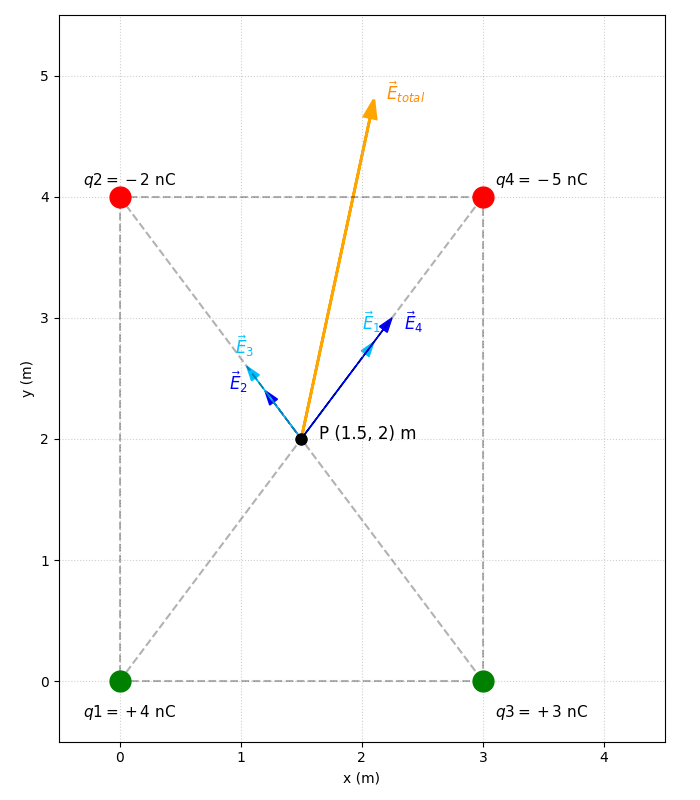
\includegraphics[width=14cm]{imagenes/2-1.png}
						\caption{Configuración de los campos eléctricos.}
					\end{figure} 
				}

			\item Calculad los campos eléctricos creados por cada carga en el punto $P$, y el campo eléctrico total, indicando dirección y sentido.

				{ \color{blue} 
					Para encontrar los campos eléctricos puntuales aplicaremos la Fórmula 11 del libro: 
					$$\vec{E}(\vec{r}) = \frac{1}{4\pi\varepsilon_0} \frac{Q}{|\vec{r} - \vec{r}'|^2} \hat{u}_{\vec{r}-\vec{r}'}$$

					Calcularemos primero la distancia $|\vec{d}_i| = |\vec{r} - \vec{r}_i|$ para cada carga. Como el punto $P$ está en el centro, la distancia es idéntica en los cuatro casos:
					$$|\vec{d}_i| = \sqrt{(\pm 1,5)^2 + (\pm 2)^2} = \sqrt{2,25 + 4} = 2,5 \text{ m}$$

					Calculamos ahora el valor de cada campo. Para ello, nos apoyamos en este valor constante común a todos: $\frac{1}{4\pi\varepsilon_0} \approx 8,99 \times 10^9 \text{ N}\cdot\text{m}^2/\text{C}^2$:

					\begin{enumerate}
						\item Carga $\mathbf{q_1 = +4 \text{ nC}}$:
							$$\hat{u}_1 = \frac{1,5}{2,5}\vec{i} + \frac{2}{2,5}\vec{j} = 0,6\vec{i} + 0,8\vec{j}$$
							$$\vec{E}_1 = (8,99 \cdot 10^9) \frac{4\cdot 10^{-9}}{2,5^2} (0,6\vec{i} + 0,8\vec{j}) \approx \boxed{3,45 \vec{i} + 4,60 \vec{j} \text{ N/C}}$$

						\item Carga $\mathbf{q_2 = -2 \text{ nC}}$
							$$\hat{u}_2 = \frac{1,5}{2,5}\vec{i} - \frac{2}{2,5}\vec{j} = 0,6\vec{i} - 0,8\vec{j}$$
							$$\vec{E}_2 = (8,99 \cdot 10^9) \frac{-2\cdot 10^{-9}}{2,5^2} (0,6\vec{i} - 0,8\vec{j}) \approx \boxed{-1,73 \vec{i} + 2,30 \vec{j} \text{ N/C}}$$

						\item Carga $\mathbf{q_3 = +3 \text{ nC}}$
							$$\hat{u}_3 = \frac{-1,5}{2,5}\vec{i} + \frac{2}{2,5}\vec{j} = -0,6\vec{i} + 0,8\vec{j}$$
							$$\vec{E}_3 = (8,99 \cdot 10^9) \frac{3\cdot 10^{-9}}{2,5^2} (-0,6\vec{i} + 0,8\vec{j}) \approx \boxed{-2,59 \vec{i} + 3,45 \vec{j} \text{ N/C}}$$

						\item Carga $\mathbf{q_4 = -5 \text{ nC}}$
							$$\hat{u}_4 = \frac{-1,5}{2,5}\vec{i} - \frac{2}{2,5}\vec{j} = -0,6\vec{i} - 0,8\vec{j}$$
							$$\vec{E}_4 = (8,99 \cdot 10^9) \frac{-5\cdot 10^{-9}}{2,5^2} (-0,6\vec{i} - 0,8\vec{j}) \approx \boxed{4,32 \vec{i} + 5,76 \vec{j} \text{ N/C}}$$
					\end{enumerate}

					Al aplicar el principio de superposición $\vec{E}_T = \sum \vec{E}_i$ (Fórmula 22), obtenemos el \textbf{campo eléctrico total} sumando los vectores correspondientes:
					$$\vec{E}_{T} = (3,45 - 1,73 - 2,59 + 4,32)\vec{i} + (4,60 + 2,30 + 3,45 + 5,76)\vec{j}$$
					$$\boxed{\vec{E}_{T} = 3,45 \vec{i} + 16,11 \vec{j} \text{ N/C}}$$

					La dirección y sentido del campo total apunta diagonalmente hacia el \textbf{primer cuadrante} al tener ambas componentes cartesianas \textbf{positivas}.
				}

			\vspace{0.5cm}

			\item Calculad la fuerza que experimentaría una carga $q_5 = -7 \; \mu$C situada en $P$.

				{ \color{blue} 
					Según la Fórmula (111), si situamos una carga dentro de un espacio con un campo eléctrico, esta se verá sometida a una fuerza definida por la ley $\vec{F} = q \cdot \vec{E}(\vec{r})$. 

					Para calcular la fuerza que recae sobre $q_5$, multiplicamos el valor de la carga en culombios ($q_5 = -7 \times 10^{-6} \text{ C}$) por el campo eléctrico total obtenido en el apartado anterior:
					$$\vec{F} = (-7 \times 10^{-6} \text{ C}) \cdot (3,45 \vec{i} + 16,11 \vec{j} \text{ N/C})$$
					$$\boxed{\vec{F} = -2,41 \times 10^{-5} \vec{i} - 1,13 \times 10^{-4} \vec{j} \text{ N}}$$

					Tal como se explica en los materiales, al tratarse de una carga de signo negativo ($q_5 < 0$), \textbf{la fuerza experimentará la misma dirección que el campo eléctrico total que actúa sobre ella, pero en sentido estrictamente contrario}. Esto se refleja en el resultado al presentar ambas componentes vectoriales de signo negativo.
				}
		\end{enumerate}
	\end{problem}

	 % --- Exercise 3 ---
	\begin{problem}[Cuestión 3]
		Abrid el simulador que encontraréis en \hyperref{https://aulaquest.com/s/fisica/campo-electrico/index.php}{este enlace}, y situad las cargas $q_1$, $q_2$ y $q_3$ de la Cuestión 2:

		\begin{itemize}
			\item $q_1 = +4 \text{ nC en } \vec{r}_1 = 0 \vec{i} + 0 \vec{j} \text{ m}$
			\item $q_2 = -2 \text{ nC en } \vec{r}_2 = 0 \vec{i} + 4 \vec{j} \text{ m}$
			\item $q_3 = +3 \text{ nC en } \vec{r}_3 = 3 \vec{i} + 0 \vec{j} \text{ m}$
		\end{itemize}

		\vspace{0.5cm}

		\begin{enumerate}[label=\alph*)] 
			\item Simulad la configuración de la cuestión 2. Realizad una captura de pantalla en la que solo se vean las líneas de campo y las líneas equipotenciales. Insertadla en vuestra hoja de respuestas.

				{ \color{blue} 
					\begin{figure}[H]
						\centering
						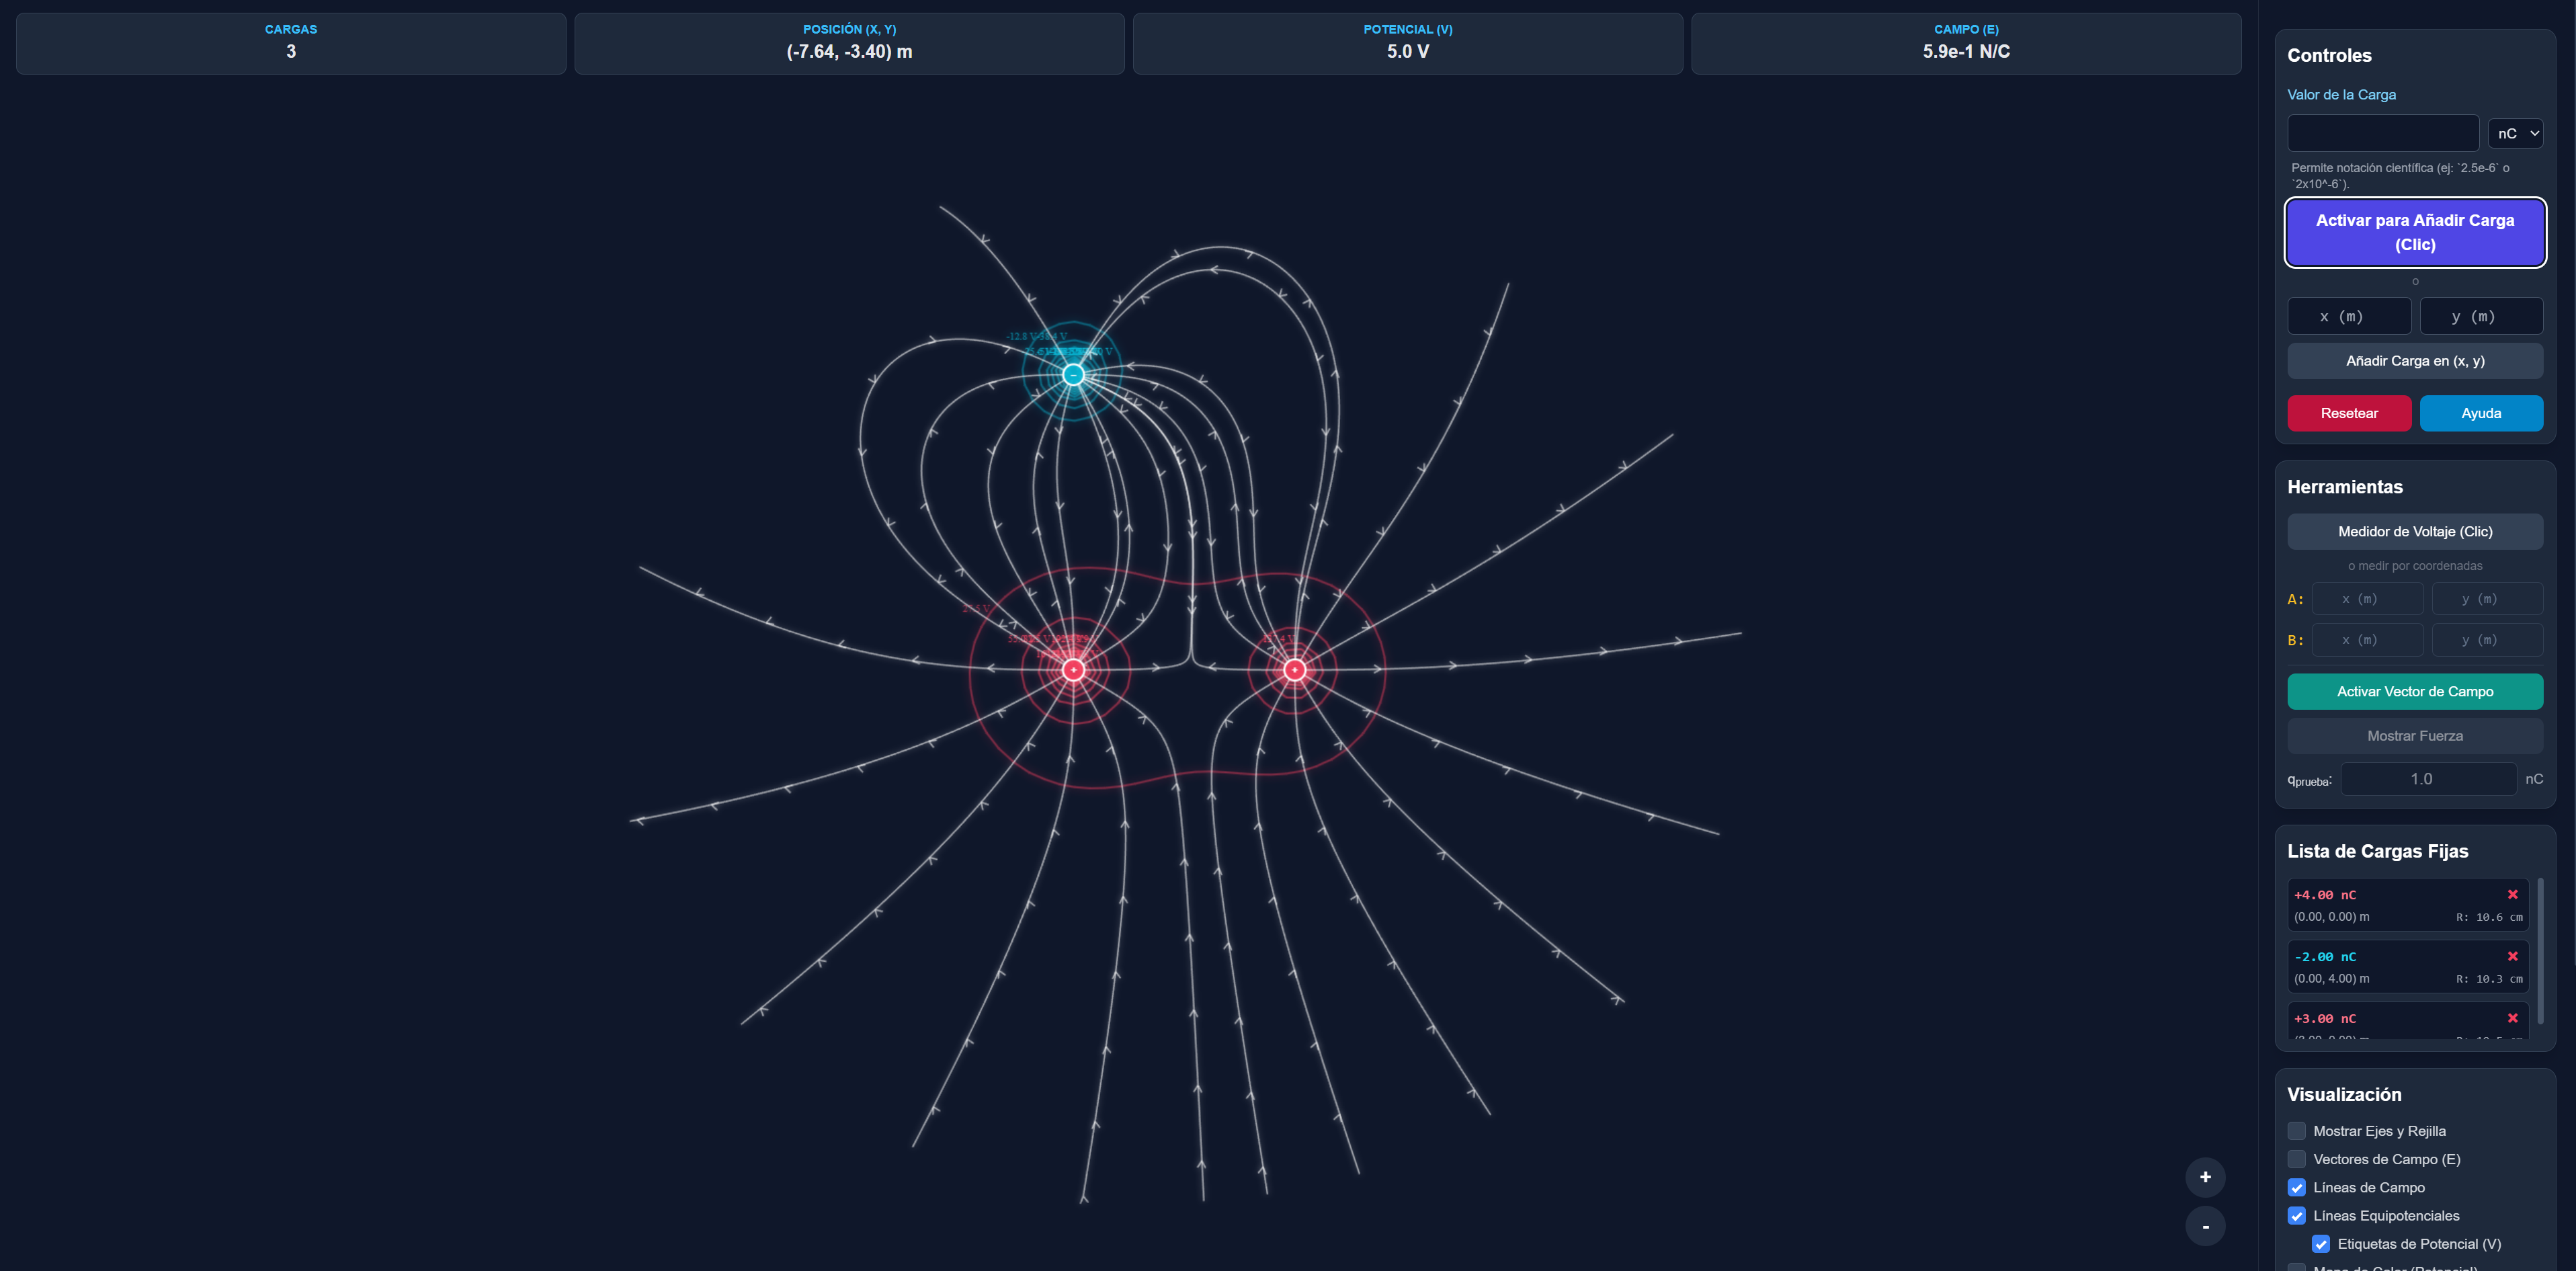
\includegraphics[width=14cm]{imagenes/3-1.png}
						\caption{Simulación de la configuración de la cuestión 2.}
					\end{figure} 
				}

			\item Explicad cómo son las líneas, por dónde entran y salen, si están juntas o separadas y explicad qué significa esto físicamente, de acuerdo con lo explicado en el módulo.

				{ \color{blue} 
					Las líneas de campo eléctrico siempre nacen de las cargas positivas, que actúan como "manantiales", y viajan por el espacio hasta morir en las cargas eléctricas negativas, que actúan como "sumideros". Las líneas que no encuentran una carga opuesta en sus proximidades se extienden hacia el infinito. Como podemos observar en las flechas direccionales de las líneas blancas, estas respetan estrictamente esta regla fundamental.

					En la simulación se aprecia que las líneas de campo están muy juntas entre sí en las proximidades inmediatas de las cargas. Físicamente, la densidad de las líneas de campo en una zona del espacio es directamente proporcional al módulo o magnitud del campo eléctrico. Por tanto, el hecho de que estén tan juntas significa que la intensidad del campo eléctrico es muy elevada cerca de las partículas. A medida que se alejan de las cargas, las líneas se van abriendo y separando progresivamente, lo que indica visualmente cómo la fuerza del campo electrostático se debilita con la distancia. Además, estas líneas de campo nunca se cruzan, ya que un cruce implicaría dos valores direccionales distintos para el campo en un mismo punto, lo cual no es posible.

					Asimismo, la imagen muestra las curvas cerradas que rodean las cargas, conocidas como líneas equipotenciales, las cuales unen todos los puntos del espacio que se encuentran a un mismo potencial eléctrico. Físicamente, estas líneas siempre son estrictamente perpendiculares a las líneas de campo eléctrico en cualquier punto de intersección y nunca se cruzan. De manera análoga a las líneas de campo, se puede observar que allí donde las líneas equipotenciales están más juntas y concentradas, la variación del potencial es mucho más brusca, lo que confirma que en esa región el campo eléctrico es más intenso.
				}

			\item Cambiad la $q_1$ situada en $\vec{r}_1 = 0 \vec{i} + 0 \vec{j}$ m por una de valor $q \prime_1 = +4 \mu$C. Pegad la captura de pantalla y explicad cómo cambian las líneas de campo respecto al apartado a).

				{ \color{blue} 
					\begin{figure}[H]
						\centering
						
\includegraphics[width=14cm]{imagenes/3-3.png}
						\caption{Simulación de la configuración con el valor de $q_1$ modificado ($\mu$C).}
					\end{figure} 

					Físicamente, la magnitud del campo eléctrico es directamente proporcional al valor de la carga que lo genera, tal como establece la Fórmula 10 del libro. Al multiplicar la cantidad de carga de $q_1$ por mil, el campo eléctrico que esta genera se vuelve inmensamente superior al que generan las otras dos cargas del sistema ($q_2$ y $q_3$), las cuales permanecen en el orden de unos pocos nanoculombios. 

					Visualmente, esta dominancia de $q_1$ se refleja en la imagen mediante la inmensa cantidad y densidad de líneas de campo (líneas blancas con flechas) que emergen del origen. De acuerdo con la teoría, la concentración o densidad de las líneas de campo es un indicador proporcional del módulo de la intensidad del campo eléctrico. Al ser $q_1$ una carga positiva de gran magnitud, actúa como un potentísimo "manantial", ya que prácticamente todas las líneas nacen de ella y apuntan de manera radial hacia el exterior. 

					El efecto de las otras dos cargas queda totalmente eclipsado por este campo masivo, motivo por el cual el patrón general de las líneas en la simulación ha perdido la interacción curva del apartado a) y ha pasado a asemejarse enormemente al de una única carga puntual positiva aislada, disparando sus líneas en línea recta hacia el infinito en todas las direcciones.
				}

			\vspace{8cm}

			\item Vuelve a cambiar la misma carga a $q\prime\prime_1 = -4 n$C. Pegad la captura de pantalla y explicad los cambios respecto al apartado a).

				{ \color{blue} 
					\begin{figure}[H]
						\centering
						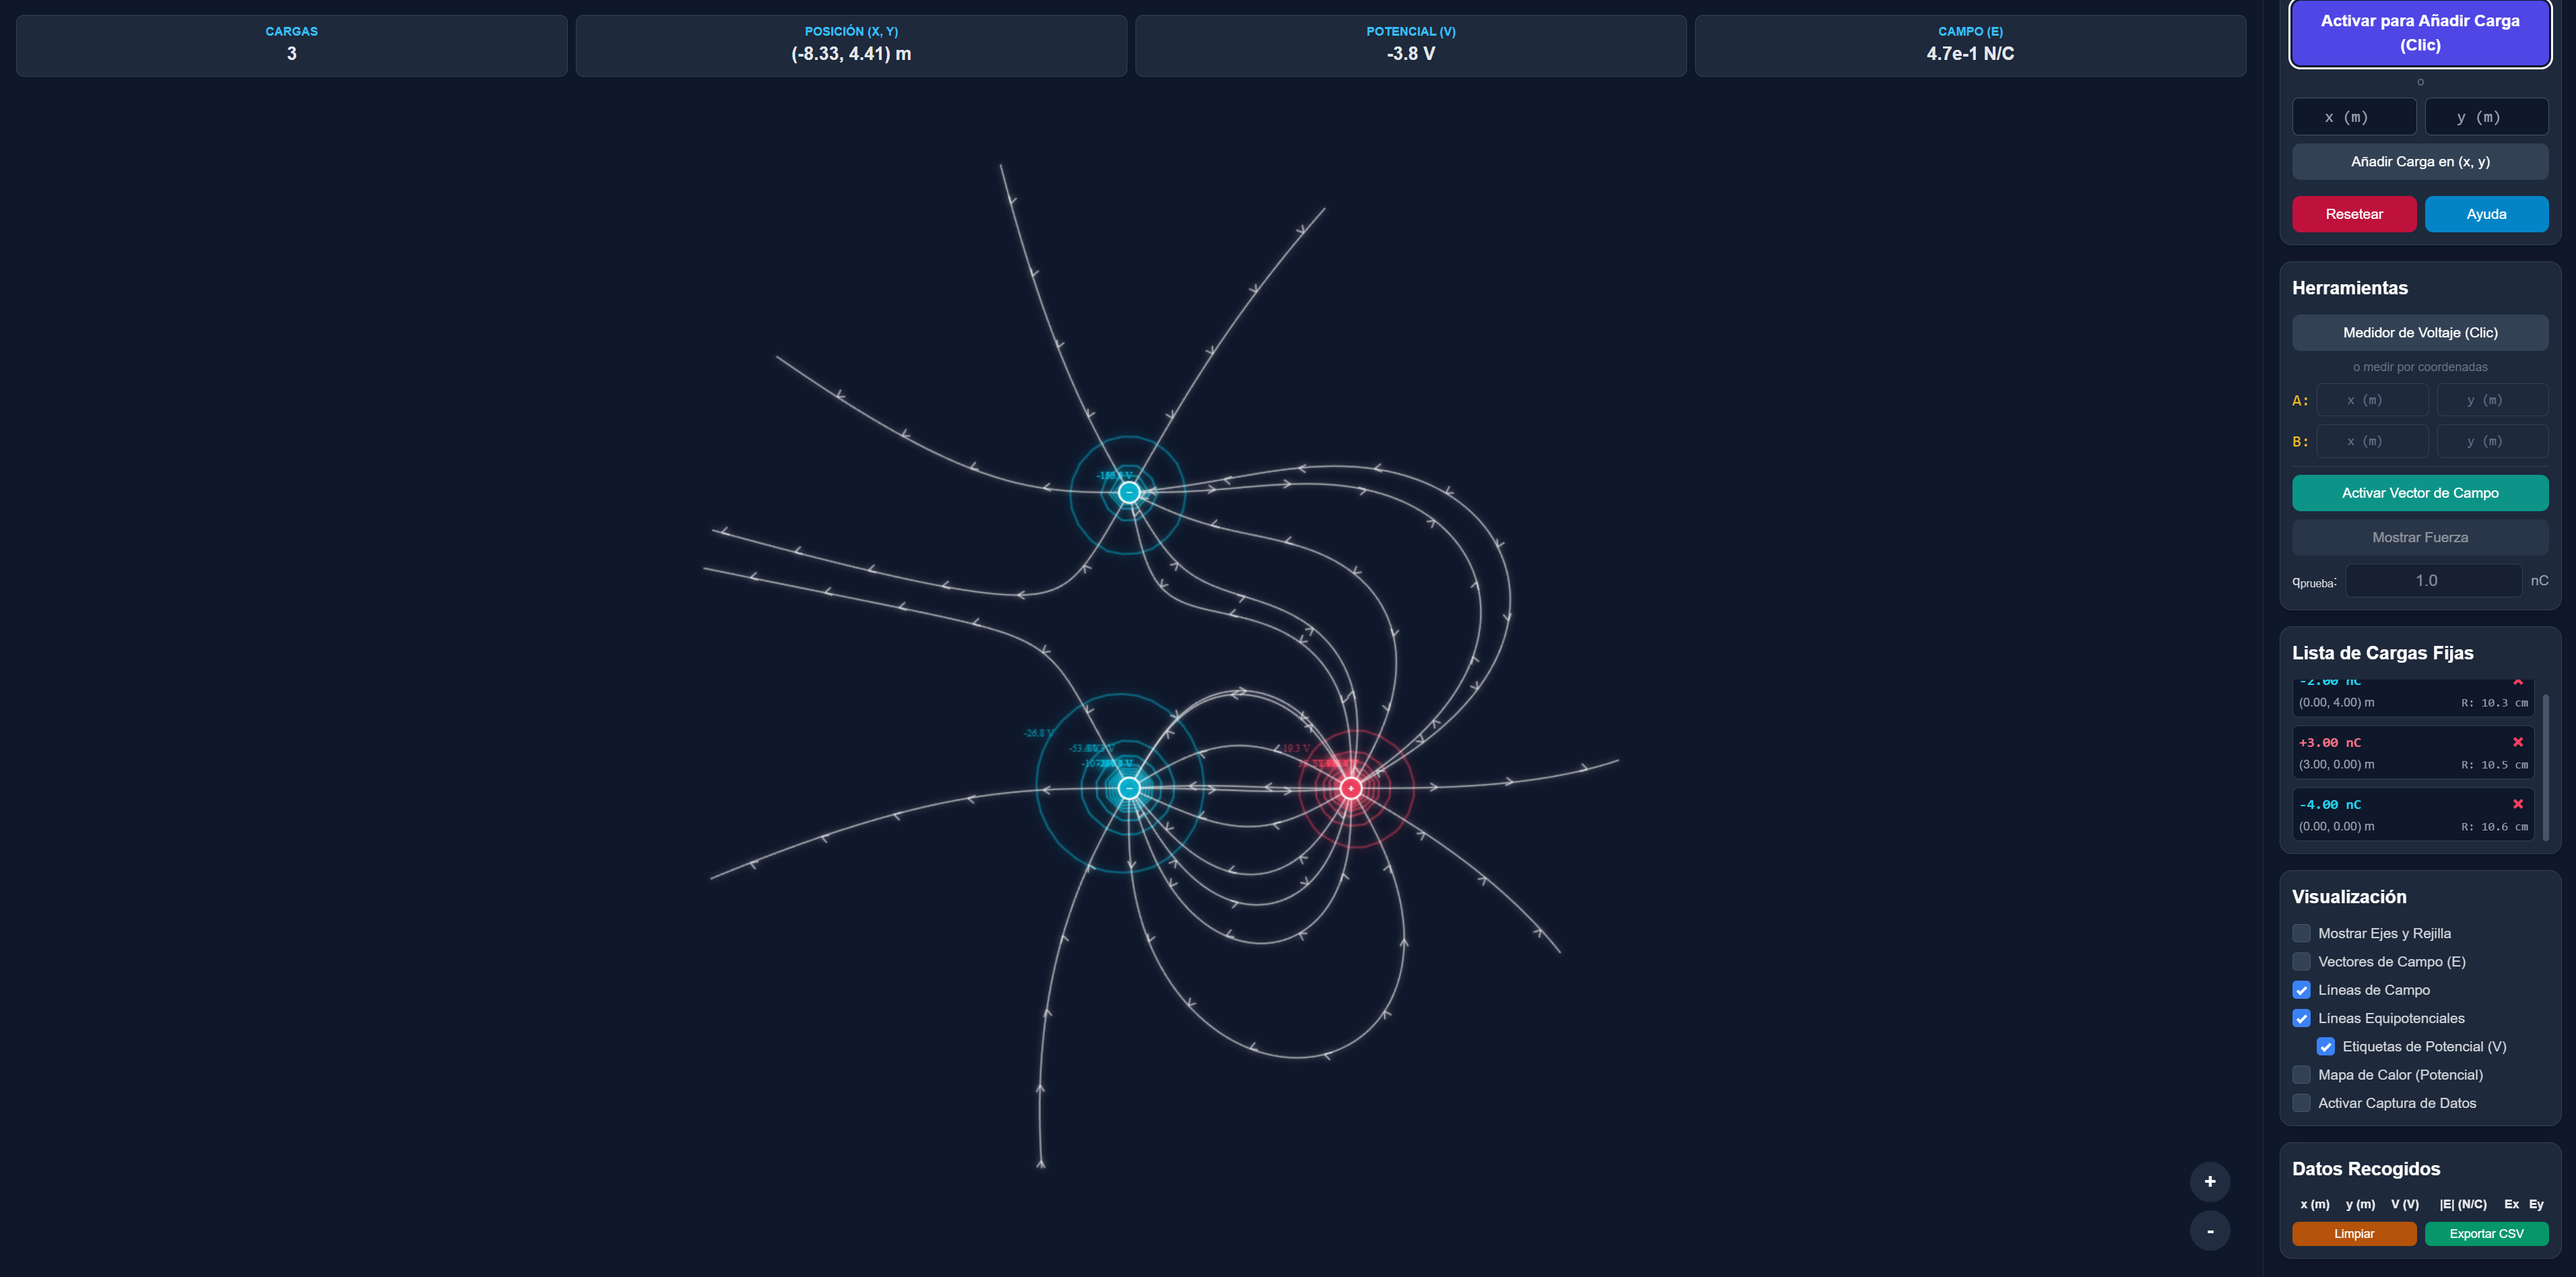
\includegraphics[width=14cm]{imagenes/3-4.png}
						\caption{Simulación de la configuración con el valor de $q_1$ modificado (negativo).}
					\end{figure} 

					En el apartado a), $q_1$ era una carga positiva y actuaba como un manantial del cual emanaban líneas de campo hacia el exterior. Ahora, al tener un valor negativo de $-4 \text{ nC}$, $q_1$ ha pasado a actuar como un "sumidero" que atrae las líneas de campo. 

					Como resultado de este cambio de polaridad, la carga $q_3$ queda como la única carga positiva de todo el sistema. Tal y como refleja claramente la Figura 3, todas las líneas de campo del sistema nacen ahora de la carga $q_3$. Desde esta única fuente positiva, las líneas se separan y viajan por el espacio para ir a morir hacia las dos cargas negativas del sistema: una parte de las líneas entra en la carga $q_2$ y la otra parte entra hacia el origen donde ahora se ubica $q_1$.
				}
		\end{enumerate}
	\end{problem}

	% --- Exercise 4 ---
	\begin{problem}[Cuestión 4]
		Tenemos una esfera conductora hueca de radio interior $R_1 = 5$ cm y radio exterior $R_2 = 7$ cm, cargada con $Q = 8$ nC.

		\begin{figure}[H]
			\centering
			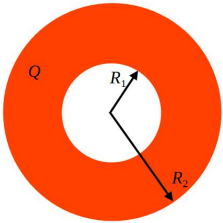
\includegraphics[width=5cm]{imagenes/enunciados/4-enunciado.png}
			\caption{Corte transversal en 2D de la esfera conductora hueca.}
		\end{figure} 

		\begin{enumerate}[label=\alph*)] 
			\item ¿Cómo se distribuyen las cargas en la esfera? Representad en la figura dónde están las cargas. ¿Será una densidad superficial o volúmica?

				{ \color{blue} 
					\begin{figure}[H]
						\centering
						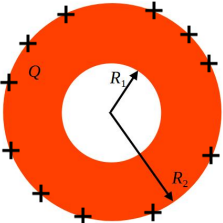
\includegraphics[width=5cm]{imagenes/4-1.png}
						\caption{Representación de las cargas en la esfera conductora hueca.}
					\end{figure} 

					Como se trata de un material conductor en equilibrio electrostático, la carga neta no puede residir en su interior, ya que el campo eléctrico interno se anula. Por lo tanto, en un conductor, toda la carga neta se redistribuye y se sitúa exclusivamente en las superficies. En este caso hueco sin carga interior, las repulsiones mutuas desplazan toda la carga $Q$ hacia la superficie exterior del conductor. 

					Como podemos ver en la Figura 5, representamos las cargas dibujando pequeños signos ``$+$'' distribuidos uniformemente a lo largo de toda la circunferencia exterior$R_2$. Dado que las cargas se acumulan únicamente sobre la frontera superficial exterior, hablaremos de una \textbf{densidad superficial de carga $\sigma$}.
				}

			\item Calculad la densidad de carga.

				{ \color{blue} 
					Para una distribución sobre una superficie, utilizamos la densidad superficial de carga $\sigma$, que equivale a la carga por unidad de superficie. Según la Fórmula 6 de los materiales, al ser uniforme, se calcula como $\sigma = \frac{Q}{S}$. 

					Dado que toda la carga está en la superficie esférica exterior, el área de cálculo es la de una esfera de radio $R_2 = 7 \text{ cm} = 0,07 \text{ m}$, es decir, $S = 4\pi R_2^2$.

					Sustituimos los valores en el Sistema Internacional:
					$$Q = 8 \text{ nC} = 8 \times 10^{-9} \text{ C}$$
					$$S = 4\pi (0,07)^2 \approx 0,06157 \text{ m}^2$$
					$$\sigma = \frac{8 \times 10^{-9} \text{ C}}{4\pi (0,07 \text{ m})^2} \approx 1,299 \times 10^{-7} \text{ C/m}^2 = 0,13 \; \mu\text{C/m}^2$$
					$$\boxed{\sigma= 0,13 \; \mu\text{C/m}^2}$$
				}

			\item Para calcular el flujo del campo eléctrico mediante el teorema de Gauss, ¿qué superficie de Gauss utilizaríais? Justificad la respuesta.

				{ \color{blue} 
					Para aplicar correctamente el teorema de Gauss, la superficie más adecuada es una \textbf{superficie esférica} concéntrica a la distribución de carga. 

					La justificación radica en la simetría esférica del problema. Sabemos que el campo eléctrico generado tiene dirección puramente radial. Al escoger una superficie de Gauss que también es una esfera, conseguimos que el vector campo eléctrico $\vec{E}$ y el vector diferencial de superficie $d\vec{S}$ (perpendicular a la superficie) sean paralelos en todos los puntos. Por tanto, forman un ángulo $\theta = 0^{\circ}$, lo que convierte el producto escalar de la integral en un producto simple ($E \cdot dS \cdot \cos(0^{\circ}) = E \cdot dS$).

					Además, a una misma distancia radial $r$, el módulo del campo $E$ es constante, lo cual permite que salga de la integral de flujo para simplificar los cálculos a $\oint E \cdot dS = E \cdot 4\pi r^2$.
				}

			\item Utilizad el teorema de Gauss para calcular el módulo del campo eléctrico en los siguientes puntos del espacio:

				\begin{itemize}
					\item $r < R_1$
					\item $R_1 < r < R_2$
					\item $R_2 < r$
				\end{itemize}

				{ \color{blue} 
					Aplicaremos la Ley de Gauss para una superficie esférica, la cual es expresada matemáticamente en la Fórmula 96: $\oint_{S} \vec{E} \cdot d\vec{S} = \frac{Q_{int}}{\varepsilon_0}$. Para nuestra geometría, el lado izquierdo de la igualdad resulta siempre en $E \cdot 4\pi r^2$. Analizamos las tres zonas:

					\textbf{1. En la zona $r < R_1$:}
					La superficie de Gauss de radio $r$ se encuentra en la cavidad vacía central. Al no haber ninguna carga encerrada en este interior, $Q_{int} = 0$. 

					Aplicando la igualdad: $E \cdot 4\pi r^2 = 0 \implies \boxed{E = 0 \text{ \textbf{N/C}}}$.

					\textbf{2. En la zona $R_1 < r < R_2$:}
					Nos ubicamos en el interior de la masa del material de la cáscara conductora. Debido a la reconfiguración de cargas descrita anteriormente, todo conductor en equilibrio electrostático mantiene un campo eléctrico nulo en su interior. 

					Alternativamente, al tomar una superficie de Gauss aquí, $Q_{int} = 0$ ya que toda la carga se ha ido a la frontera $R_2$. Por tanto: $\boxed{E = 0 \text{ \textbf{N/C}}}$.

					\textbf{3. En la zona $R_2 < r$:}
					La superficie de Gauss en este caso envuelve a toda la esfera conductora hueca, por lo que la carga neta total encerrada es $Q_{int} = Q = 8 \times 10^{-9} \text{ C}$. 

					Igualamos los términos según la ley de Gauss (Fórmula 100):
					$$E \cdot 4\pi r^2 = \frac{Q}{\varepsilon_0} \implies E = \frac{Q}{4\pi\varepsilon_0 r^2}$$

					Sustituimos el valor de $Q$ y de la constante $\frac{1}{4\pi\varepsilon_0} \approx 8,99 \times 10^9 \text{ N}\cdot\text{m}^2/\text{C}^2$:
					$$\boxed{{\mathbf{E}} = (8,99 \times 10^9) \frac{8 \times 10^{-9}}{r^2} = \mathbf{\frac{71,92}{r^2} \text{ \textbf{N/C}}}}$$ (expresando $r$ en metros)
				}
		\end{enumerate}
	\end{problem}

	% -- Exercise 5 ---
	\begin{problem}[Cuestión 5]
		Tres cargas de valores $q_1 = q_3 = +5$ nC y $q_2 = -5$ nC están colocadas en el espacio tal como se ve en la Figura 2, con $a = 10$ cm.

		\begin{figure}[H]
			\centering
			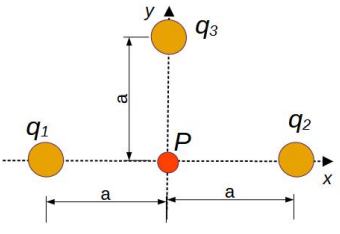
\includegraphics[width=10cm]{imagenes/enunciados/5-enunciado.png}
			\caption{Fuerzas eléctricas sobre la carga $Q$ en el punto $P$}
		\end{figure} 

		\begin{enumerate}[label=\alph*)] 
			\item Calculad el potencial en el punto $P$.

				{ \color{blue} 
					Para calcular el potencial eléctrico en el punto $P$, aplicamos el principio de superposición sumando los potenciales creados por cada carga individualmente, usando la Fórmula 145 de los materiales: $V = \sum_{i=1}^{N} \frac{1}{4\pi\varepsilon_0} \frac{Q_i}{|\vec{r} - \vec{r}'_i|}$. 

					Si observamos la figura del enunciado, podemos apreciar que el punto $P$ se ubica en el cruce de los ejes, por lo que la distancia desde cada una de las tres cargas hasta $P$ es exactamente $a = 10 \text{ cm} = 0,1 \text{ m}$.

					Sustituimos los valores en la fórmula y sumamos las contribuciones de $q_1$, $q_2$ y $q_3$:
					$$V_P = V_1 + V_2 + V_3 = \frac{1}{4\pi\varepsilon_0} \left( \frac{q_1}{a} + \frac{q_2}{a} + \frac{q_3}{a} \right)$$

					Dado que $q_1 = +5 \text{ nC}$ y $q_2 = -5 \text{ nC}$, sus contribuciones al potencial se anulan exactamente al sumarlas: 
					$$\frac{5 \times 10^{-9}}{0,1} + \frac{-5 \times 10^{-9}}{0,1} = 0$$

					Por lo tanto, el potencial total en $P$ dependerá únicamente de la carga $q_3$:
					$$V_P = \frac{1}{4\pi \cdot 8,85 \times 10^{-12}} \frac{5 \times 10^{-9}}{0,1} \approx 8,99 \times 10^9 \cdot 50 \times 10^{-9} = 449,5 \text{ V}$$
					$$\boxed{V_P = 449,5 \text{ V}}$$
				}

			\item Situamos una carga $Q=+10$ nC en el punto $P$. Calculad su energía.

				{ \color{blue} 
					Para encontrar la energía potencial eléctrica adquirida por una carga al ubicarla en un punto con un potencial conocido, empleamos la Fórmula 143: 

					$$\Delta U = Q \cdot V(\vec{r})$$

					Dado que consideramos el origen del potencial en el infinito, donde la energía es nula, la energía del sistema se calcula multiplicando directamente el valor de la nueva carga instalada por el potencial que hemos obtenido en el apartado anterior:
					$$U = Q \cdot V_P = (10 \times 10^{-9} \text{ C}) \cdot 449,5 \text{ V} = 4,495 \times 10^{-6} \text{ J} = 4,495 \; \mu\text{J}$$
					$$\boxed{U = 4,495 \; \mu \text{J}}$$
				}

			\item Dibujad el sistema y señalad la dirección y el sentido de la fuerza eléctrica sobre la carga $Q$ en el dibujo, justificando la respuesta (no es necesario realizar el cálculo).

				{ \color{blue} 
					\begin{figure}[H]
						\centering
						
\includegraphics[width=10cm]{imagenes/5c.png}
						\caption{Situación de las cargas de la Cuestión 5.}
					\end{figure} 

					Al situar la carga de prueba $Q$ en el origen, experimenta tres fuerzas individuales que debemos sumar vectorialmente según el principio de superposición.

					En el eje horizontal, la carga $q_1$ ejerce una fuerza de repulsión $\vec{F}_1$ que empuja a $Q$ hacia la derecha. A su vez, la carga $q_2$ ejerce una fuerza de atracción $\vec{F}_2$ que también tira de $Q$ hacia la derecha. Por lo tanto, en el eje X, ambas fuerzas se suman creando una componente de magnitud considerable en el sentido positivo del eje X.

					En el eje vertical, la carga $q_3$ ejerce una fuerza de repulsión $\vec{F}_3$ que empuja a $Q$ hacia abajo, en el sentido negativo del eje Y.

					Cuando sumamos vectorialmente la componente horizontal total y la componente vertical, el vector de la fuerza eléctrica neta ($\vec{F}_{neta}$) se origina en $P$ y apunta diagonalmente hacia el cuarto cuadrante.
				}
		\end{enumerate}
	\end{problem}

		% -- Exercise 6 ---
	\begin{problem}[Cuestión 6]
		Indicad si las afirmaciones siguientes son ciertas (C) o falsas (F). En todos los casos, \textbf{justificad} brevemente la respuesta.

		\begin{enumerate}[label=\alph*)] 
			\item En un dieléctrico sometido a un campo eléctrico, las cargas libres se desplazan a través del material.

				{ \color{blue} 
					\textbf{Falsa (F).} Un dieléctrico es un material aislante que no tiene cargas libres que puedan desplazarse a través de él. Los átomos están fijados en su estructura, por lo que al someterse a un campo eléctrico externo, lo que ocurre es una ligera separación o reorganización de las cargas internas que crean pequeños dipolos eléctricos locales, pero no hay un flujo o desplazamiento de cargas libres en el material.
				}

			\item La polarización de un dieléctrico reduce el campo eléctrico efectivo dentro del material.

				{ \color{blue} 
					\textbf{Cierta (C).} La polarización produce pequeños dipolos eléctricos dentro del material que generan un campo eléctrico interno ($\vec{E}_p$) con sentido opuesto al campo eléctrico externo aplicado ($\vec{E}_q$). Por consiguiente, el campo eléctrico total o efectivo dentro del dieléctrico ($\vec{E}_i$) disminuye, lo cual se describe mediante la relación $E_i = E_q - E_p$ (Fórmula 225). Esto también se puede cuantificar de forma que el campo en el interior se reduce en un factor correspondiente a la permitividad relativa: $E_i = \frac{E_{\text{vacío}}}{\varepsilon_r}$ (Fórmula 226).
				}

			\item Al introducir un dieléctrico entre las placas de un condensador conectado a una fuente, la carga almacenada aumenta.

				{ \color{blue} 
					\textbf{Cierta (C).} Al llenar el condensador con un material dieléctrico, su capacidad se multiplica por la permitividad relativa del material según la fórmula $C = \varepsilon_r C_{\text{vacío}}$ (Fórmula 228). Dado que el condensador está conectado a una fuente, la diferencia de potencial ($\Delta V$) en sus bornes se mantiene constante. Según la definición de capacidad mostrada en la Fórmula 204 ($C = \frac{Q}{\Delta V}$), la carga puede calcularse como $Q = C \cdot \Delta V$. Si la capacidad ($C$) es mayor y el voltaje es fijo, la cantidad de carga almacenada ($Q$) debe aumentar forzosamente.
				}
		\end{enumerate}
	\end{problem}

	% --- Problem ---
	\begin{problem}[Problema]
		En una placa base de un ordenador se coloca un condensador plano formado por dos placas con las siguientes características:

		\begin{itemize}
			\item Área: $2 \text{ cm}^2$
			\item Separación: $0.5 \text{ mm}$
			\item Dieléctrico: $\varepsilon_r = 4$
		\end{itemize}

		Está conectado a 5 V. Calculad:

		\begin{enumerate}[label=\alph*)] 
			\item La capacidad del condensador $C_1$.

				{ \color{blue} 
					Para calcular la capacidad de un condensador plano-paralelo con un dieléctrico, utilizamos la Fórmula 228 del libro, $C = \varepsilon_r C_{vacio}$, donde la capacidad en el vacío es $C_{vacio} = \frac{\varepsilon_0 S}{d}$ según la Fórmula 205. 

					Sustituyendo los valores en unidades del Sistema Internacional:
					$$C_1 = 4 \cdot \frac{8,85 \times 10^{-12} \text{ F/m} \cdot 2 \times 10^{-4} \text{ m}^2}{0,5 \times 10^{-3} \text{ m}} = 1,416 \times 10^{-11} \text{ F} = \mathbf{14,16 \text{ \textbf{pF}}}$$
					$$\boxed{C_1 = 14,16 \text{ pF}}$$
				}

			\item La carga y energía almacenadas.

				{ \color{blue} 
					La carga almacenada se calcula mediante la definición general de capacidad (Fórmula 204): $Q = C \cdot \Delta V$.
					$$Q_1 = (14,16 \times 10^{-12} \text{ F}) \cdot 5 \text{ V} = 7,08 \times 10^{-11} \text{ C} = 70,8 \text{ pC}$$
					$$\boxed{Q_1 = 70,8 \text{ pC}}$$

					La energía almacenada se obtiene con la Fórmula 206: $U = \frac{1}{2} C \cdot \Delta V^2$.
					$$U_1 = \frac{1}{2} (14,16 \times 10^{-12} \text{ F}) \cdot (5 \text{ V})^2 = 1,77 \times 10^{-10} \text{ J} = 177 \text{ pJ}$$
					$$\boxed{U_1 = 177 \text{pJ}}$$
				}

			\item El campo entre placas y fuera de las placas.

				{ \color{blue} 
					Para calcular el campo \textbf{entre las placas}, relacionamos la diferencia de potencial con el campo eléctrico utilizando la Fórmula 227, de la que se deduce que $E = \frac{\Delta V}{d}$.
					$$\boxed{E = \frac{5 \text{ V}}{0,5 \times 10^{-3} \text{ m}} = 10000 \text{ V/m}}$$ (o N/C)

					\textbf{Fuera de las placas}, de acuerdo con las deducciones mostradas en la Figura 38 y la Fórmula 199, los campos eléctricos generados por la placa positiva y negativa tienen el mismo módulo pero sentidos contrarios, por lo que su suma es nula. Por lo tanto, $E_{fuera} = \mathbf{0 \text{ \textbf{V/m}}}$.
				}

			\item La densidad superficial de cargas en las placas.

				{ \color{blue} 
					La densidad superficial de carga $\sigma$ se obtiene dividiendo la carga almacenada entre la superficie de la placa (Fórmula 202): $\sigma = \frac{Q}{S}$.
					$$\sigma = \frac{70,8 \times 10^{-12} \text{ C}}{2 \times 10^{-4} \text{ m}^2} = 3,54 \times 10^{-7} \text{ C/m}^2 = 0,354 \; \mu\text{C/m}^2$$
					$$\boxed{\sigma = 0,354 \; \mu\text{C/m}^2}$$
				}

			\item Si dejáramos una carga de $-5 \; \mu$C en el punto medio entre las placas, ¿a qué fuerza se vería sometida y en qué sentido? ¿Y si la dejáramos fuera de las placas?

				{ \color{blue} 
					Según la ley de Coulomb descrita en la Fórmula 111, la fuerza eléctrica que experimenta una carga es $\vec{F} = q \cdot \vec{E}$ [8].

					\textbf{En el punto medio entre las placas}, el módulo de la fuerza será $F = |-5 \times 10^{-6} \text{ C}| \cdot 10000 \text{ V/m} = \mathbf{0,05 \text{ \textbf{N}}}$. 

					Como la carga insertada tiene signo negativo, la fuerza experimentará la misma dirección pero en \textbf{sentido contrario} al del campo eléctrico que actúa sobre ella. En otras palabras: la fuerza se dirigirá hacia la placa cargada positivamente.

					En el caso de fuera de las placas, como el campo eléctrico exterior es nulo ($E_{fuera} = 0 \text{ V/m}$), la fuerza que experimentará la carga también será nula: $\mathbf{0 \text{ \textbf{N}}}$.
				}

			\item Ahora, conectamos el condensador en serie con otro de igual geometría pero con el vacío como dieléctrico $C_2$, y los extemos conectados a 5 V. Dibujad el esquema del circuito y calculad. ¿Cuál será la tensión de cada uno de los condensadores? \textit{(NOTA: considerad que los dos condensadores están inicialmente descargados)}.

				{ \color{blue} 
					\begin{figure}[H]
						\centering
						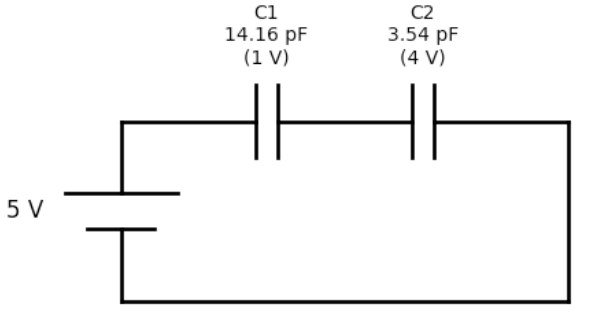
\includegraphics[width=10cm]{imagenes/problema-1.jpg}
						\caption{Esquema del circuito en serie}
					\end{figure} 

					Primero determinamos la capacidad de $C_2$ (vacío) mediante la Fórmula 205:
					$$C_2 = \frac{\varepsilon_0 S}{d} = \frac{14,16 \text{ pF}}{4} = 3,54 \text{ pF}$$

					La capacidad equivalente $C_e$ en serie se calcula con la Fórmula 218:
					$$\frac{1}{C_e} = \frac{1}{14,16} + \frac{1}{3,54} \implies C_e = 2,832 \text{ pF}$$

					En una asociación en serie, todos los condensadores adquieren la misma carga, equivalente a la total del sistema (Fórmula 237):
					$$Q_1 = Q_2 = Q_e = C_e \cdot V_{total} = 2,832 \text{ pF} \cdot 5 \text{ V} = 14,16 \text{ pC}$$

					Las tensiones de cada condensador se aíslan con la Fórmula 204:
					$$\boxed{V_1 = \frac{Q_1}{C_1} = \frac{14,16 \text{ pC}}{14,16 \text{ pF}} = {1 \text{ V}}}$$
					$$\boxed{V_2 = \frac{Q_2}{C_2} = \frac{14,16 \text{ pC}}{3,54 \text{ pF}} = 4 \text{ V}}$$
				}

			\item Partiendo del condensador $C_1$ cargado con 5 V del apartado b), lo conectamos en paralelo con el segundo condensador $C_2$, descargado inicialmente, sin conexión a ninguna fuente de alimentación. Dibujad el esquema del circuito.

				{ \color{blue} 
					\begin{figure}[H]
						\centering
						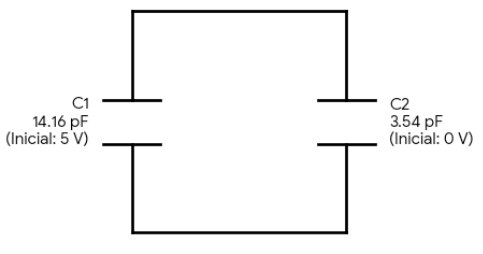
\includegraphics[width=10cm]{imagenes/problema-2.jpg}
						\caption{Esquema de condensadores en paralelo (sin fuente)}
					\end{figure} 
				}

			\item Calculad la carga y los voltajes de cada uno de los condensadores del apartado anterior una vez estabilizados.

				{ \color{blue} 
					Puesto que no hay fuentes externas y la carga no puede escapar, rige el principio de conservación de la carga . La carga total del sistema será la que $C_1$ poseía originalmente en el apartado b), ya que $C_2$ estaba vacío:
					$$Q_{tot} = 70,8 \text{ pC}$$

					Al conectarlos en paralelo, la capacidad equivalente es la suma de las dos capacidades individuales (Fórmula 224):
					$$C_p = C_1 + C_2 = 14,16 \text{ pF} + 3,54 \text{ pF} = 17,7 \text{ pF}$$

					En un sistema paralelo estabilizado, todos los elementos comparten un mismo voltaje. Lo calculamos para el sistema equivalente aislando la tensión (Fórmula 262):
					$$\boxed{V' = \frac{Q_{tot}}{C_p} = \frac{70,8 \text{ pC}}{17,7 \text{ pF}} = 4 \text{ V}}$$ 

					Este será el voltaje tanto para $C_1$ como para $C_2$.

					Con el nuevo voltaje común, obtenemos la nueva carga distribuida en cada condensador (Fórmulas 263 y 264):
					$$\boxed{Q_1' = C_1 \cdot V' = 14,16 \text{ pF} \cdot 4 \text{ V} = 56,64 \text{ pC}}$$
					$$\boxed{Q_2' = C_2 \cdot V' = 3,54 \text{ pF} \cdot 4 \text{ V} = 14,16 \text{ pC}}$$
				}
		\end{enumerate}
	\end{problem}
\end{document}